\section{FAB-MAP 1.0}

\subsection{Overview}
\begin{frame}{Overview (Key Elements)}
    \begin{itemize}
        \item Probabilistic
        \item Based on visual bag of words (BoW)
        \item Capture the co-occurence of words
        \item New places VS places already in the map
        \item O($n_{places}$), while previously done in O($n_{places}^3$)
        \item Processing in real time for thousands of places
    \end{itemize}
    \note[item]{Section: Overview}
    \note[item]{Probabilistic based framework}
    \note[item]{Bag of visual Words (SURF, k-means)}
    \note[item]{Complexity of ...}
    \note[item]{Capture co-occurence in unsupervised way using CLT}
    \note[item]{Can differentiate new places from place already in the map}
\end{frame}

\subsection{Approximating High-Dimensional Discrete Distributions}
\begin{frame}{Approximating Distributions}
    \begin{itemize}
        \item Goal: approximate high-dimensional discrete distributions
        \item $P(Z)$, where $Z=\{z_1,z_2,...,z_n\}$
        \item P(Z) general representation is exponential in $n$
        \item Approximate $P(Z)$ by $Q(Z)$
        \item Similarity metric: Kullback-Leibler
            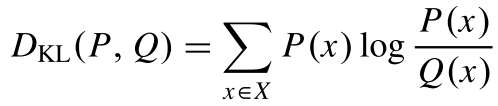
\includegraphics[width=0.6\textwidth]{./media/kullback_leibler.png}
    \end{itemize}
    \note[item]{Goal here: approximate high-dimensional discrete distributions}
    \note[item]{Probability distribution on n discrete variables (z: notation for observation, binary word)}
    \note[item]{P(Z) the general distribution without structure, exponential in n = intractable}
    \note[item]{You want to approximate P(Z) by Q(Z) with a special structure = tractable}
    \note[item]{To maximize the similarity between the distribution: Kullback-Leibler}
    \note[item]{Zero when equal, strictly positive else (want to minimize that distance)}
\end{frame}

\begin{frame}{Approximating Distributions}
    \begin{itemize}
        \item Naive Bayes: each variable must be independent
        \item Alternative: each variable is conditioned on at most one other variable
            \begin{itemize}
                \item Restricts the graphical model of Q(Z) to be a tree
                \item $n^{(n-2)}$ possible graphical model
                \item \textbf{Chow Liu Tree}
            \end{itemize}
    \end{itemize}
    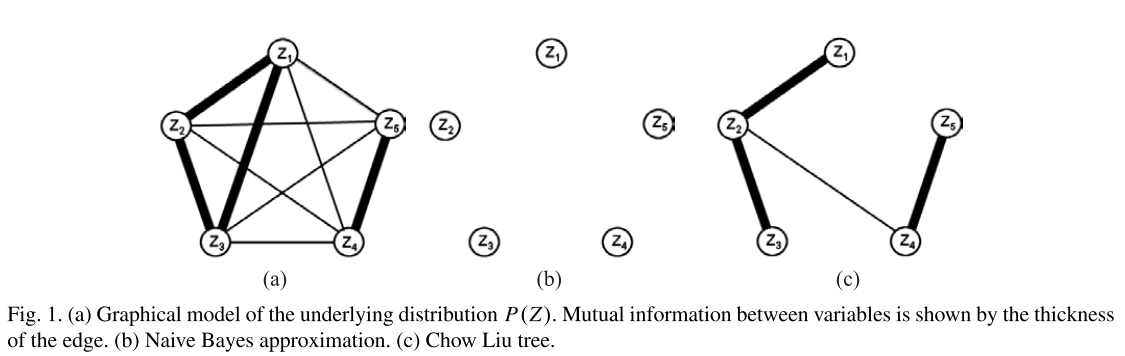
\includegraphics[width=1.0\textwidth]{./media/chow_liu_tree.png}

    \note[item]{Naive Bayes: example, $Q(Z)$ is restricted such that each variable must be independent}
    \note[item]{Naive Bayes: tractable, independent variables, single possible configuration}
    \note[item]{A less severe constraint: each variable in Q(Z) is conditioned on at most one other variable}
    \note[item]{CLT described a polynomial time algorithm to select the best such distribution}
\end{frame}

\subsection{Probabilistic Navigation Using Appearance}
\begin{frame}{Representing Locations}
    \begin{itemize}
        \item At time $k$, there is $n_k$ discrete locations $\mathcal{L}^k=\{L_1,...,L_{n_k}\}$
        \item Instead of using directly $P(Z|L_j)$:
            \begin{itemize}
                \item Introduce hidden variable $e_i$: the event that an object which generates observations of type $z_i$ exist
                \item Location model: $\{p(e_1=1|L_i),...,p(e_{|v|}=1|L_i)\}$
                \item A detector model relates feature existence $e_i$ to feature detection $z_i$.
                    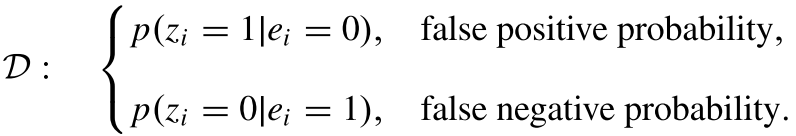
\includegraphics[width=0.7\textwidth]{./media/detector.png}
                \item Each of the feature generating objects $e_i$ are generated independently by the location
            \end{itemize}
    \end{itemize}
    \note[item]{Now I will talk about the Probabilistic Navigation Using Appearance}
    \note[item]{First I will explain how they represent a location}
    \note[item]{}
    \note[item]{Rather than model each of the locations directly in terms of which features are likely to be observed}
    \note[item]{Model each location as a set...}
\end{frame}

\begin{frame}{Representing Locations}
    \begin{columns}
        \begin{column}{0.7\textwidth}
            Reasons for $e$:
            \begin{enumerate}
                \item Natural framework for incorporating data from multiple sensors
                \item It facilitate factoring the distribution $p(Z|L_j)$ into two parts% — a simple model for each location composed of independent variables $e_i$ , and a more complex model that captures the correlations between detections of appearance words $p(z_i|Z_k)$
            \end{enumerate}
        \end{column}

        \begin{column}{0.3\textwidth}
            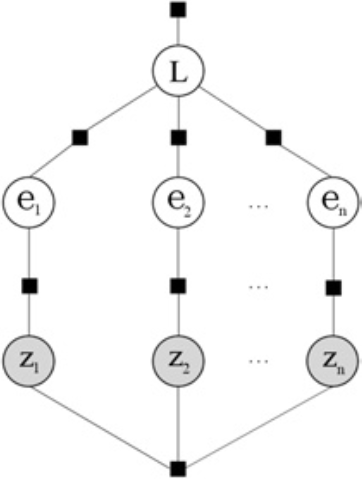
\includegraphics[width=\textwidth]{./media/event.png}
        \end{column}
    \end{columns}
    \note[item]{You can see a representation of the model on the right}
    \note[item]{They say they are 2 reasons to introduce the hidden variable}
    \note[item]{Natural framework for incorporating data from multiple sensors}
    \note[item]{It facilitate factoring the distribution $p(Z|L_j)$ into two parts}
    \note[item]{a simple model for each location composed of independent variables $e_i$}
    \note[item]{and a more complex model that captures the correlations between detections of appearance words $p(z_i|Z_k)$}
\end{frame}

\begin{frame}{Estimating Location via Recursive Bayes}
    Calculating $p(L_i|\mathcal{Z}^{k})$ can be formulated as a recursive Bayes estimation problem:
    \begin{equation*}
        p(L_i|\mathcal{Z}^{k}) = \frac{p(Z_k|L_i,\mathcal{Z}^{k-1})p(L_i|\mathcal{Z}^{k-1})}{p(Z_k|\mathcal{Z}^{k-1})}
    \end{equation*}
    \begin{itemize}
        \item Prior belief: $p(L_i|\mathcal{Z}^{k-1})$
        \item Observation likelihood: $p(Z_k|L_i,\mathcal{Z}^{k-1})$
        \item Normalizing term: $p(Z_k|\mathcal{Z}^{k-1})$
    \end{itemize}
    \vspace{0.5cm}
    Assumption: $p(Z_k|L_i,\mathcal{Z}^{k-1}) = p(Z_k|L_i)$
    \note[item]{We first assume independence between the current and past observations}
    \note[item]{It can be evaluate as discussed in previous slides... == NB or CLT}
\end{frame}

\begin{frame}{New Place or Old Place ?}
    \begin{itemize}
        \item Normalization term only deal with localization\\ \vspace{0.3cm}
            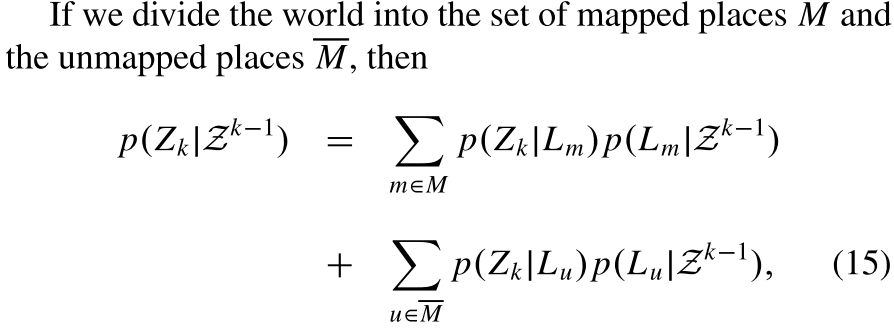
\includegraphics[width=0.7\textwidth]{./media/nomalize_new.png}
        \item Second summation involves all possible unknown places.
        \item Compared 2 different approximations:
            \begin{enumerate}
                \item Mean field
                \item Sampling (Monte Carlo)
            \end{enumerate}
    \end{itemize}
    \note[item]{Normalization have to be modified to deal with new places}
    \note[item]{Second summation cannot be evaluated directly because it involves all possible unknown places}
    \note[item]{Mean field: L="average place", e=marginal probability}
    \note[item]{Select random image from a large collection of observations}
\end{frame}

\begin{frame}{Location Prior}
    \begin{itemize}
        \item Location prior: $p(L_i|Z^{k-1})$
        \item Use motion model
        \item Robot at place $i$ at time $t$ is likely to be at \{$i-1$, $i$, $i+1$\} at time $t+1$
        \item Places with unknown neighbours ?
        \item Could be improved, but they found that effect of the prior is weak
    \end{itemize}
    \note[item]{Motion model: not building topological map, they assume sequentially collected observations}
    \note[item]{Equal probability for i-1 i and i+1}
    \note[item]{When unknown neighbours, part of the probability mass assigned to a "new place" node}
    \note[item]{The remainder is spread evenly over all places}
    \note[item]{Could be improved, but they found that effect of the prior is weak}
\end{frame}

\begin{frame}{Smoothing}
    \begin{itemize}
        \item Performance on the inference is strongly dependent on the normalizing term
        \item Fully capture the visual variety of the environment
        \item Very slight smoothing of the data likelihood values
        \item Reject most outliers, still allows loop closure after 2-3 corresponding images
    \end{itemize}
    \note[item]{To fully capture the visual variety of environment, large set of place models... need time and data}
    \note[item]{Workaround, Smoothing prevent asserting loop closure with high confidence for single image pair}
    \note[item]{2-3 corresponding images and hop !}
\end{frame}

\begin{frame}{Parameters}
    User-specified inputs:
    \begin{itemize}
        \item Detector model: $p(z_i=1|e_i=0)$ and $p(z_i=0|e_i=1)$
        \item The smoothing parameter ($\sigma$)
        \item Prior probability that a topological link with an unknown endpoint leads to a new place
    \end{itemize}
\end{frame}

\subsection{Results}
\begin{frame}{Results}
    \begin{itemize}
        \item Chow Liu tree built from 2800 images from 28 km (10 meters apart)
        \item Vocabulary of approximately 11000 words
        \item 2 hours on 3Ghz Pentium IV
        \item Detector model: $p(z_i=1|e_i=0)=0$ and $p(z_i=0|e_i=1)=0.39$
        \item The smoothing parameter: $\sigma=0.99$
        \item Prior probability that a topological link with an unknown endpoint leads to a new place: 0.9
    \end{itemize}
    \note[item]{Section: Results}
    \note[item]{Chow Liu tree built from 2800 images from 28 km (10 meters apart)}
    \note[item]{Vocabulary of approximately 11000 words}
    \note[item]{2 hours on 3Ghz Pentium IV}
    \note[item]{Detector model: $p(z_i=1|e_i=0)=0$ and $p(z_i=0|e_i=1)=0.39$}
    \note[item]{The smoothing parameter: $\sigma=0.99$}
    \note[item]{Prior probability that a topological link with an unknown endpoint leads to a new place: 0.9}
\end{frame}

\begin{frame}{Word Examples}
    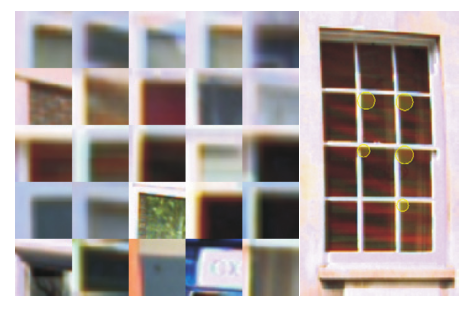
\includegraphics[width=0.5\textwidth]{./media/word_top_left.png}
    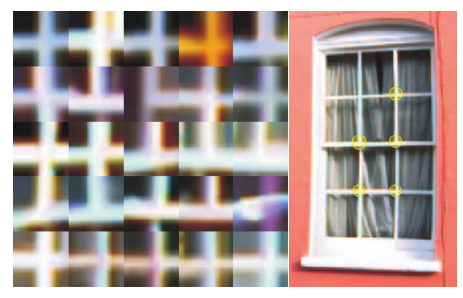
\includegraphics[width=0.5\textwidth]{./media/word_bot_right.png}
    \note[item]{Left most correlated with right and vice versa}
\end{frame}

\begin{frame}{Results}
    \begin{itemize}
        \item Two outdoor datasets
            \begin{enumerate}
                \item New College: perceptual aliasing
                \item City Center: presence of scene changes (dynamic objects, light changes)
            \end{enumerate}
        \item Show results using Chow Liu tree and Monte Carlo (best results)
        \item Goal: 100\% precision
        \item Recall of 48\% for New College and 37\% for City Center
    \end{itemize}
\end{frame}

\begin{frame}{New College}
    \begin{center}
        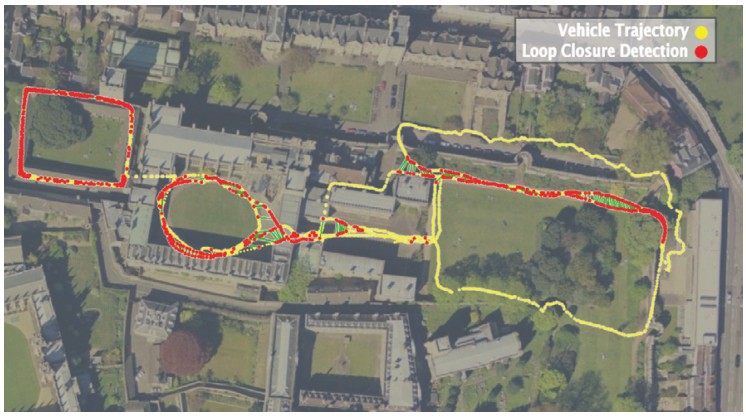
\includegraphics[width=0.9\textwidth]{./media/new_college.png}
    \end{center}
\end{frame}

\begin{frame}{City Center}
    \begin{center}
        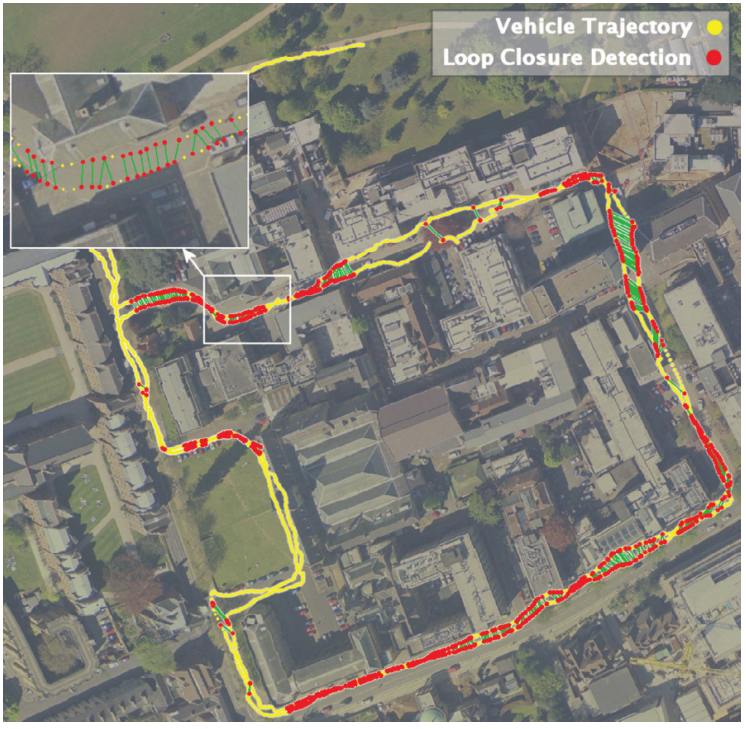
\includegraphics[width=0.6\textwidth]{./media/city_center.png}
    \end{center}
\end{frame}

\begin{frame}{Perceptual Aliasing}
    \begin{center}
        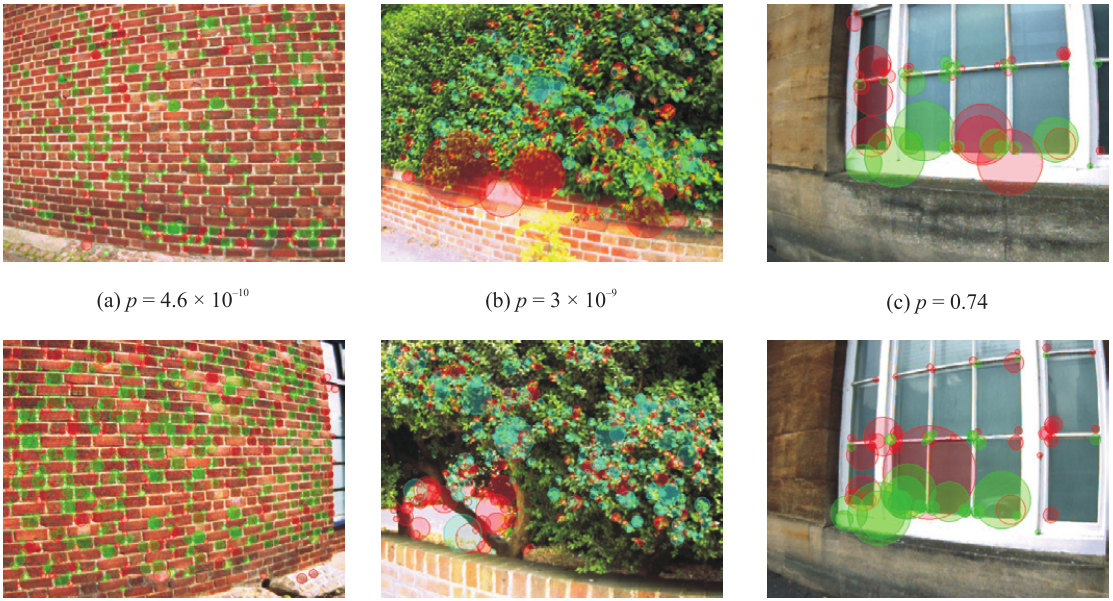
\includegraphics[width=0.9\textwidth]{./media/perceptual_aliasing.png}
    \end{center}
    \note[item]{Recognized with as low as 8\%, reject with as much as 45\%.}
    \note[item]{Threshold they use is 99\%}
\end{frame}

\begin{frame}{Comparing Approximations}
    \begin{center}
        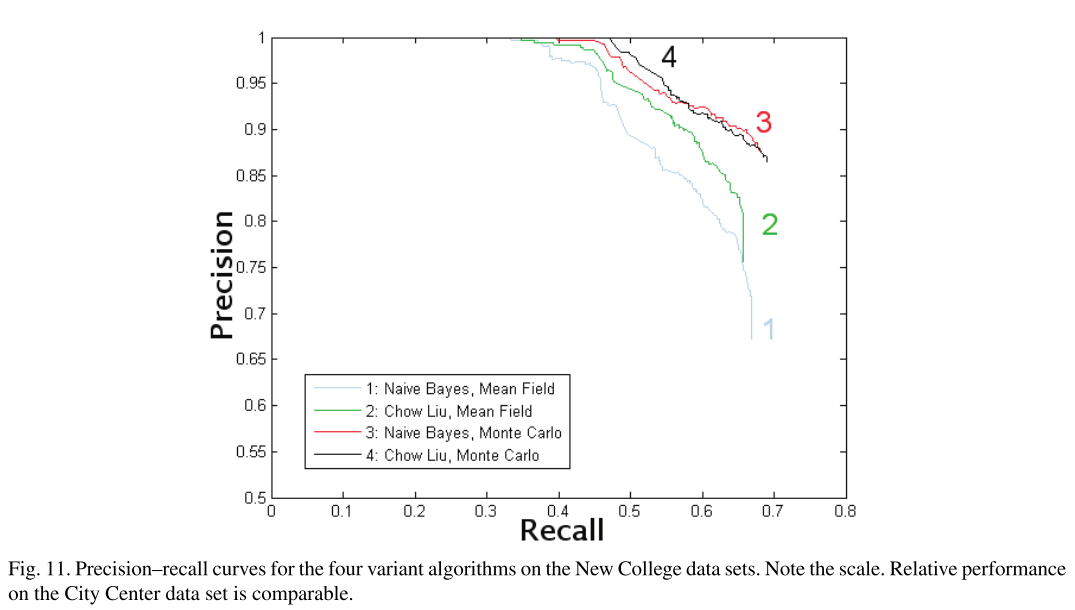
\includegraphics[width=\textwidth]{./media/compare_fig.png}
    \end{center}
\end{frame}

\begin{frame}{Comparing Approximations}
    \begin{center}
        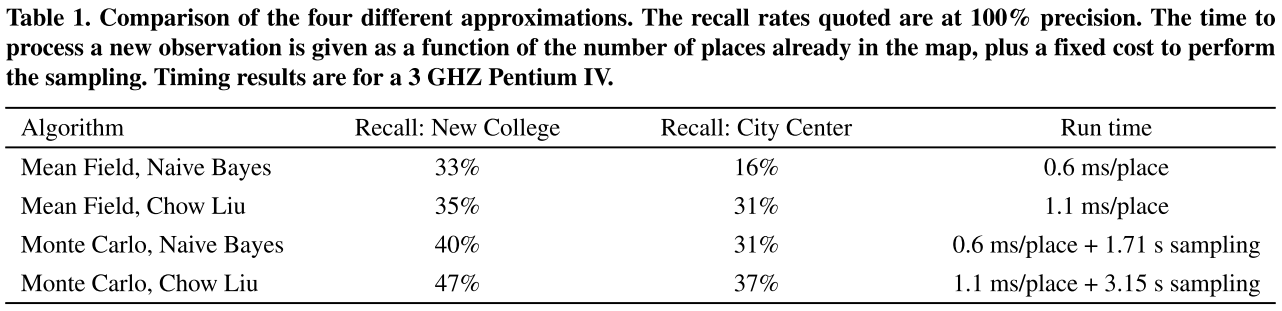
\includegraphics[width=\textwidth]{./media/table.png}
    \end{center}
\end{frame}
